\subsubsection{MySQL (Handle)}
MySQL ist eine der bekanntesten und weit verbreiteten relationalen Datenbankverwaltungssystem auf der Welt. Ursprünglich wurde es von MySQL AB entwickelt, wurde jedoch von Sun Microsystems übernommen und ist jetzt in Händen von Oracle. Es ist als Open-Source Software oder als kommerzielle Enterprise Version verfügbar.\\
\paragraph{SQL}
Dieses Datenbankmanagementsystem verwendet als Sprache für den Zugriff auf die Datenbank SQL.\\
SQL steht für \textbf{Structured Query Language} wurde dafür entwickelt eine einheitliche und leicht lesbare Programmierschnittstelle zur Verfügung zu stellen, um Datenbanken zu bearbeiten.\\
SQL ist eine Datenbanksprache für relationale Datenbanken. Sie kann dazu verwendet werden Datenbanken und Tabellen zu erstellen und bearbeiten und Datensätze zu Bearbeiten, damit ist löschen, ändern oder einfügen von Datensätzen in Tabellen gemeint. Außerdem können auch Datensätze abgefragt werden  und können auch gefiltert, sortiert und vieles mehr werden. Die Voraussetzung ist, dass das Datenbanksystem auf dieser Datenbanksprache basiert.\\
Hier die wichtigisten Befehle die verwendet wurden.\\
\subparagraph{Beispiele für Befehle}
\begin{itemize}
    \item SELECT
    	\begin{itemize}
	    	\item Mit SELECT können Datensätze aus Tabellen abgerufen werden. Zu diesem Befehl gibt es noch einige zusätze, um zum Beispiel die Daten zu filtern, zu sortieren oder Tabellen miteinander zu Verknüpfen.
	    	\begin{itemize}
		    	\item \textit{SELECT * FROM classes;}\\
		    		Damit werden alle Datensätze aus der Tabelle classes ausgelesen.
		    	\item \textit{SELECT short FROM teachers;}\\
			    	Damit wird nur die Spalte der Lehrerkürzel ausgelesen, jedoch von allen Datensätzen.
		    	\item \textit{SELECT * FROM classes WHERE name LIKE '2 \%'}\\
		    		Damit werden alle Datensätze von Klassen ausgelesen, bei denen der Name mit 2 beginnt. So erhält man alle Klassen des 2. Jahrgangs.
		    	\item \textit{SELECT * FROM substitudes ORDER BY time ASC}\\
		    		Damit werden alle Supplierungen in aufsteigender Reihenfolge(ASC) ausgelesen. Sollen die Supplierungen absteigend ausgelesen werden verwendet man statt ASC DESC.
		    	\item \textit{SELECT teachers.name FROM classes LEFT JOIN teachers ON teachers.ID = classes.teacherFK}\\
		    		Mit dieser Abfrage können alle KV's der Klassen abgefragt werden. Da im Datenbankdesign auf Redundanzvermeidung geachtet wurde, wird in der classes Tabelle auf die teachers Tabelle verwiesen. Dort stehen die Namen der KV's. In der classes Tabelle steht nur die eindeutige ID des Lehrers.\\\\
		    		\textbf{\textit{SELECT teachers.name FROM classes LEFT JOIN teachers ON teachers.ID = classes.teacherFK}}\\
		    			Gibt alle Einträge der Tabelle classes zurück, jedoch nur die Einträge von der teachers Tabelle, die die ON Bedingung erfüllen.\\\\
		    		\textbf{\textit{SELECT teachers.name FROM classes INNER JOIN teachers ON teachers.ID = classes.teacherFK}}\\
		    			Gibt nur diejenigen Datensätze zurück, die die ON Bedingung erfüllen.\\\\
		    		\textbf{\textit{SELECT teachers.name FROM classes RIGHT JOIN teachers ON teachers.ID = classes.teacherFK}}\\
		    			Gibt alle Einträge der Tabelle teachers zurück und nur die Einträge der Tabelle classes die die ON Bedingung erfüllen.\\\\
		    		\textbf{\textit{SELECT teachers.name FROM classes OUTER JOIN teachers ON teachers.ID = classes.teacherFK}}\\
		    			Gibt alle EInträge aus beiden Tabellen zurück. Die Einträge, die die ON Bedingung erfülle werden zusammengefügt und die anderen werden jeweils als einzelner Datensatz angezeigt.\\
		    	\item \textit{SELECT name as Klassenname FROM classes}\\
		    		Mit as können die Spaltennamen der Tabelle in besser lesbaren oder besser identifizierbaren Spaltennamen umbenannt werden.
	    	\end{itemize}
    	\end{itemize}
    \item INSERT
	    \begin{itemize}
		   	\item Mit dem INSERT Befehl können neue Datensätze in eine Tabelle eingefügt werden.
		   	\begin{itemize}
			   	\item \textit{INSERT INTO sections (name,short,teacherFK) VALUES ('TestAbteilung','T','2')}\\
			   		Damit wird eine neue Abteilung in der Tabelle sections erstellt. Dabei werden die angegebenen Spalten auf die in der Klammer stehenden Werte gesetzt. Hier muss die Spalte ID nicht angegeben werden, da sie auf \textit{auto increment} gesetzt ist.
		   	\end{itemize}
	    \end{itemize}
	\item UPDATE
		\begin{itemize}
			\item Mit dem UPDATE Befehl können Datensätze in einer Tabelle verändert werden.
			\begin{itemize}
				\item \textit{UPDATE sections SET name = 'TestAbteilung2' WHERE name = 'TestAbteilung'}\\
					Mit diesem UPDATE Befehl wird jeder Datensatz der in der Spalte name TestAbteilung stehen hat abgeändert. Dabei wird TestAbteilung in TestAbteilung2 geändert.
				\item \textit{UPDATE sections SET name = 'TestAbteilung123',short = 'T123' WHERE name = 'TestAbteilung2'}\\
					Dies Funktioniert im Prinzip gleich wie der Befehl zuvor. Mit dem Unterschied, dass dabei 2 Spalten geändert werden.
			\end{itemize}
		\end{itemize}
	\item DELETE
		\begin{itemize}
			\item Mit DELETE können einzelne Datensätze oder auch mehrere Datensätze auf einmal gelöscht werden.
			\begin{itemize}
				\item \textit{DELETE FROM sections WHERE name = 'TestAbteilung123'}\\
					Damit werden alle Datensätze mit name = TestAbteilung123 gelöscht. Ohne dem WHERE Parameter werden alle Datensätze aus der Tabelle sections gelöscht.
			\end{itemize}
		\end{itemize}
	\item TRUNCATE
		\begin{itemize}
			\item Mit TRUNCATE können alle Datensätze aus einer Tabelle gelöscht werden. Im unterschied zu DELETE wird hier auch der Index zurückgesetzt. Bei DELETE werden die neuen Datensätze fortlaufend weiter mit dem letzten Index nummeriert. Bei TRUNCATE beginnt die Nummerierung von vorne.
			\begin{itemize}
				\item \textit{TRUNCATE FROM classes}\\
					Dabei wird die ganze Tabelle classes zurückgesetzt und damit auch alle Datensätze gelöscht. 
			\end{itemize} 
			
		\end{itemize}
\end{itemize}
\paragraph{Aufbau von MySQL}
Bei MySQL ist es im Normalfall so, dass die Datenbank/en auf einem MySQL Server liegen und die MySQL-Client/s Anfragen auf diesen Server senden.\\
Ein Server kann mehrere Datenbanken beinhalten. Eine solche Datenbank kann jeweils mehrere Tabellen beinhalten. Jede Tabelle hat mehrere Spalten.\\
Jede Spalte hat einen bestimmten Datentyp. Hier einige wichtige Datentypen, die benützt wurde:
\begin{itemize}
	\item TINYINT\\
	Wird für die Speicherung von BOOL Werten verwendet, da es den wenigsten Speicherplatz benötigt
	\item INT\\
	Wird für die Speicherung von Ganzzahlen verwendet.
	\item DATE\\
	Wird für die Speicherung von Datumsangaben verwendet.
	\item TEXT\\
	Wird für die Speicherung von Texten verwendet.
\end{itemize}
\paragraph{Verarbeitung von Anfragen}
Eine Anfrage, die an einen MySQL-Server gesendet werden, durchläuft wird grundsätzlich mit diesen Schritten abgearbeitet. Zuerst wird im Query-Cache nachgeschaut ob ein gleicher Query schon einmal gestellt wurde und ob sich die Tabelle seither nicht mehr geändert hat. Ist es ein neuer Query, dann wird der Query an den Parser gesendet und anschließend wird der Query optimiert und das Ergebnis wird zurückgeliefert.
\subparagraph{Query-Cache}
Wird ein Qery an den MySQl-Server gesendet wird zuerst im Query-Cache nachgeschaut, ob der selber Query schon einmal gestellt wurde. Ist dies der Fall, so muss noch kontrolliert werden ob sich die Daten in der Datenbank seither geändert wurden. Hat sich nichts verändert, so sendet der MySQL-Server die gespeicherten Ergebnisse zurück. Dies hat den Vorteil, dass der MySQL-Server nicht wieder den Query ausführen muss und ist somit Ressourcensparender. 
\subparagraph{Parsing}
Beim Parsing wird der gestellte Query in seine einzelnen Befehle zerlegt. Außerdem werden alle Informationen über den Query gesammelt. Wie zum Beispiel wird die Art(SELECT,DELETE,UPDATE,...) des Querys bestimmt. Ist das Parsing abgeschlossen so ist ein so genannter Parse-Baum erstellt worden. Dieser wird anschließend Optimiert.
\subparagraph{Optimierung}
In diesem Schritt wird der geparste Code optimiert. Dabei wird der Query analysiert, so werden die besten Abfragereihenfolgen ausarbeitet. Es wird bestimmt, welche Tabellen wie und wann gejoined werden. Außerdem wird kontrolliert ob alle Tabellen die im Query vorkommen auch wirklich benötigt werden.\\
Ist die optimale Abfragereihenfolge gefunden wird der Query ausgeführt und das Ergebnis wird zurückgegeben.
\paragraph{Administration}
MySQL liefert Standardmäßig einen Kommandozeilen-Client mit. Dieser kann in der Konsole mit \textit{mysql} aufgerufen werden. Damit können Datenbanken, Tabellen erstellt und bearbeitet werden, Datensätze können bearbeitet, verändert und gelöscht werden. Es können noch viele weitere Funktionen damit genutzt werden.\\
\subparagraph{Grafische Tools}
Es gibt noch zahlreiche grafische Tools MySQL Server zu administrieren. Eines der am weit Verbreitetsten grafischen Tools ist phpMyAdmin. Dies ist ein Tool, das auf einen Webserver kopiert wird und es erlaubt über ein Webinterface alle Einstellungen und Datenbankbefehle grafisch ausführen zu können. Dies erleichtert und vereinfacht das Erstellen, Bearbeiten und Verändern von Datenbanken und Tabellen. Damit können auch ungeübte Personen MySQL Datenbanken verwenden.
\paragraph{MySQL $ \Rightarrow $ PHP}
Um über PHP auf einen MySQL Server zugreifen zu können benötigt man das PHP-Modul php5-mysql, welches einige MySQL Befehle zur Verfügung stellt um mit einem MySQL-Server zu kommunizieren.\\
\subparagraph{Verbindung aufbauen}
Um mit einem MySQL-Server eine Verbindung aufzubauen müssen diese PHP Befehle verwendet werden(siehe Programm-Code \ref{lst:content_mysql_connect}).
\begin{lstlisting}[style=custom, language=PHP, caption={MySQL Connect},label={lst:content_mysql_connect}]
<?php 
	mysql_connect($host, $user, $passwd);
	mysql_select_db($db);
?>
\end{lstlisting}
Wobei in diesem Beispiel entspricht \textit{\$host} der Adresse des MySQL-Server, liegt der Webserver, von wo aus die Anfrage gesendet wird und er MySQL Server am selben Server so ist dies \textit{localhost}. \textit{\$user} ist der Usernamen zum anmelden auf dem MySQL Server und \textit{\$pass} ist das Passwort für die Anmeldung am MySQL Server. Mit \textit{\$db} wird die Datenbank angegeben mit der gearbeitet werden soll. Die Funktion \textit{mysql\_connect()} gibt im Fehlerfall FALSE zurück und im Erfolgsfall einen Ressource Wert. \textit{mysql\_select\_db()} gibt bei Erfolg TRUE zurück, sonst FALSE.
\subparagraph{Anfragen}
Um Anfragen an einen MySQL Server senden zu können muss man diesen Syntax verwenden(siehe Programm-Code \ref{lst:content_mysql_query})
\begin{lstlisting}[style=custom, language=PHP, caption={MySQL Querys},label={lst:content_mysql_query}]
<?php 
	$sql="SELECT * FROM classes";
	mysql_query($sql);
?>
\end{lstlisting}
In der unter \ref{lst:content_mysql_query} gezeigtem Programmsequenz ist eine Anfrage an den MySQL Server gezeigt. Wichtig ist, dass zuvor die Zeilen vom \autoref{lst:content_mysql_connect} stehen, damit eine Anfrage an den Server gesendet werden kann. \textit{mysql\_query} gibt bei Datenbankabfragen(SELECT, SHOW, EXPLAIN, ...) das Abfrageergebnis im Erfolgsfall zurück, bei Fehlerfall FALSE. Wird ein anderer Datenbankbefehl(INSERT, DELETE, UPDATE, ...) ausgeführt, so gibt die Funktion bei Erfolg TRUE und bei Misserfolg FALSE zurück.\\
Das Ergebnis ist in Zeilen aufgebaut, d.h. will man jede Zeile abarbeiten, muss man jede Zeile zum Beispiel mit einer do-while-Schleife durchlaufen. Ein interner Positionszeiger verweist auf die momentane Stelle. Die Funktionen zum Abfragen dieser Zeilen stellt den Zeiger immer eine Stelle weiter.\\
Das Ergebnis bei einer Abfrage ist jedoch nicht in einem Format mit dem man arbeiten kann, deshalb muss dieses Ergebnis noch an weitere Funktionen weitergegeben werden. Hier die von uns am häufigsten verwendeten Funktionen:
\begin{itemize}
	\item \textit{mysql\_fetch\_array()}
	\begin{itemize}
		\item Mit dieser Funktion wird eine Zeile des Ergebnisses gelesen und in ein Array geschriebn. Zusätzlich wird der Positionszeiger eine Stelle weiter gestellt.\\
		Die Indizes des Arrays werden nummerisch nummeriert und sind nochmals mit den Spaltennamen nummeriert. Das heißt, die Ergebnisse sind in diesem Array doppelt vorhanden 
	\end{itemize}
	\item \textit{mysql\_fetch\_object()}
		\begin{itemize}
			\item Mit dieser Funktion wird die aktuelle Zeile des Ergebnisses ausgelesen und als Objekt zurückgegeben. Iwederum wird der Positionszeiger eine Stelle weiter gestellt.
		\end{itemize}
	\item \textit{mysql\_fetch\_row()}
		\begin{itemize}
			\item Diese Funktion gibt eine Zeile des Ergebnisses als Array zurück das nummerisch nummerierte Indizes hat. Das heißt hier sind aus dem Array die Spaltennamen nicht ersichtlich. Auch hier wird der Datenzeiger um eine Stelle weiter gestellt.
		\end{itemize}
\end{itemize}
Im Programm Code \ref{lst:content_mysql_fetch_array} ist ein Ausschnitt einer Abarbeitung eines MySQL Results zu sehen. Hier wird zuerst ein Query an den Server gesendet und danach werden alle Ergebniszeilen durchlaufen und in ein Array gespeichert. Dazu wird \textit{mysql\_fetch\_array()}verwendet. Dies ist die Funktion die ich persönlich bevorzuge.\\
\begin{lstlisting}[style=custom, language=PHP, caption={MySQL Query weiterverarbeiten},label={lst:content_mysql_fetch_array}]
<?php 
	$sql = "SELECT * FROM hours LIMIT 0,5"; //Mit LIMIT wird die Abfrage auf die ersten 5 Ergebnisse begrenzt
	$result = mysql_query($sql); //Ergebnis wird in der Variable $result gespeichert
	
	while($row = mysql_fetch_array($result)){	//Jede Ergebniszeile wird durchlaufen
		$ergebnis[] = $row;	//Hier wird die Zeile in einen Eintrag des Arrays geschrieben
	}
	
	print_r($ergebnis);	//Relationale Ausgabe des Arrays mit allen Zeilen
	
?>
\end{lstlisting}
Öffnet man den Quelltext der oberen Seite, wiederum muss zuvor natürlich der Programm-Code \ref{lst:content_mysql_connect} in dem PHP Code eingefügt werden, um überhaupt eine Verbindung mit dem MySQL Server herstellen zu können, dann wird das Array \textit{\$ergebnis} schön dargestellt. Das Ergebnis ist in der Abb. \ref{fig:content_mysql_fetch_array} zu sehen.\\
Hier ist gut zu sehen, dass bei \textit{mysql\_fetch\_array()} die Spalten nummerisch und laut Spaltenname indiziert werden. Dies kann durch dem zweiten Parameter in der Funktion \textit{mysql\_fetch\_array()} geändert werden. Außerdem ist hier zu sehen, dass jede Ergebniszeile einen eigenen Index (nummerisch Nummeriert) in dem Array \textit{\$ergebnis} hat, daraus ergibt sich ein Mehrdimensionales Array.\\
Auf die erste Zeile des Ergebnisses kann also mit \textit{\$ergebnis[0]} zugegriffen werden. Das Ergebnis dieses Codes ergibt Abb. \ref{fig:content_mysql_fetch_row}. Um dann auf die Start-Uhrzeit der Stunde von der ersten Zeile zugreifen zu können, kann man entweder den nummerischen Index oder die Spaltenbezeichnung verwenden. Also entweder \textit{\$ergebnis[0][4]} oder \textit{\$ergebnis[0]['startTime']}.\\ Das Ergebnis dieser Zeilen ist dasselbe, dieses ist in Abb. \ref{fig:content_mysql_fetch_column} zu sehen.\\
\begin{figure}[H]
\centering
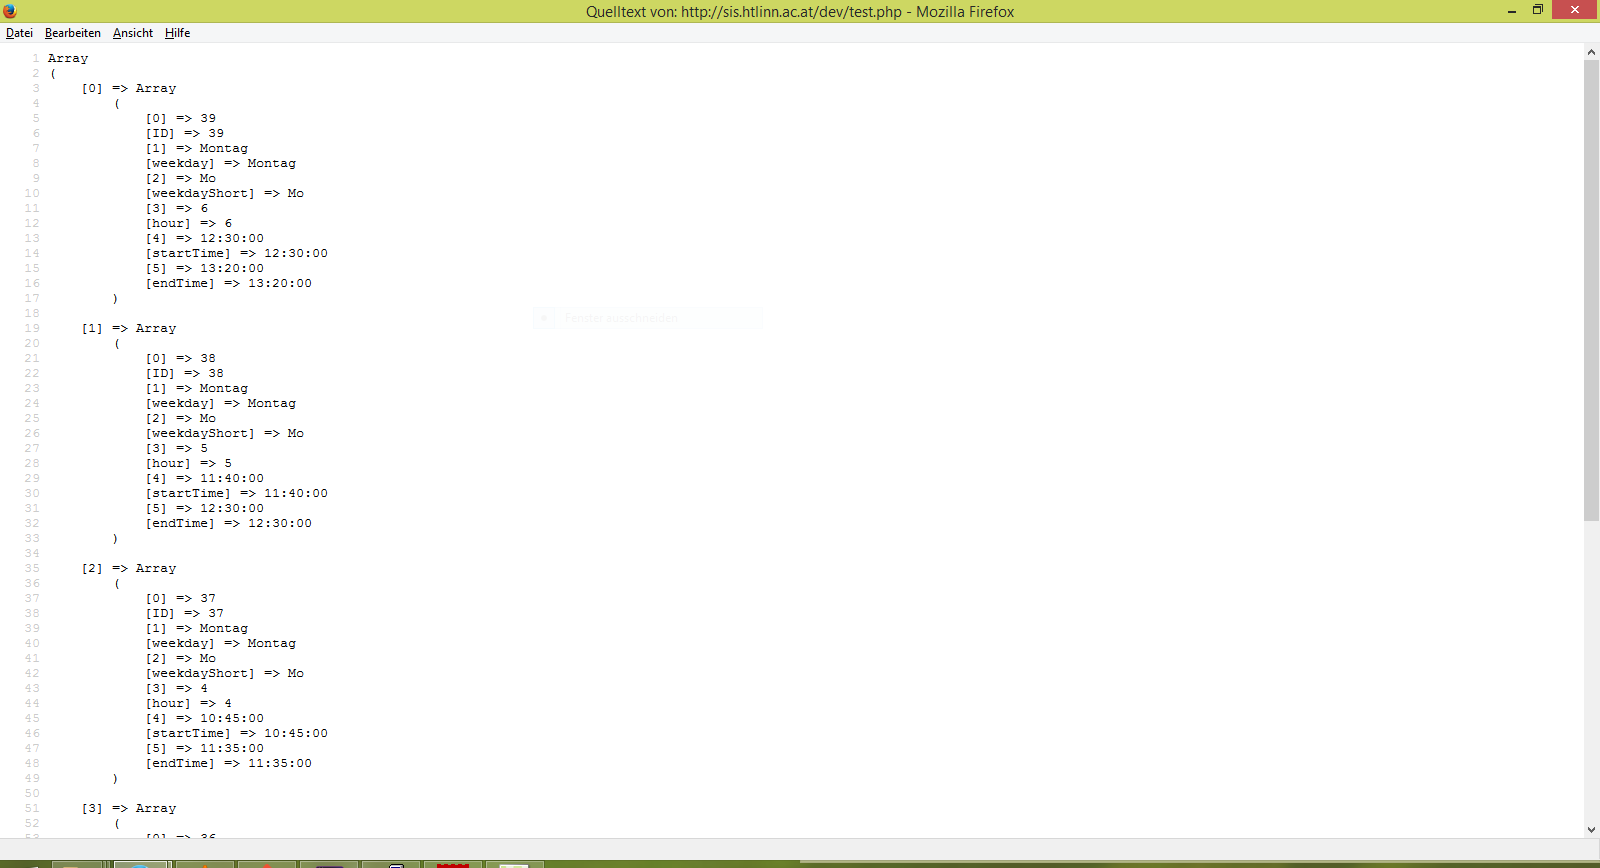
\includegraphics[keepaspectratio=true, width=14cm]{images/screenshots/content_mysql_fetch_array.png}
\caption{MySQL Fetch Array}
\label{fig:content_mysql_fetch_array}
\end{figure}
\begin{figure}[H]
\centering
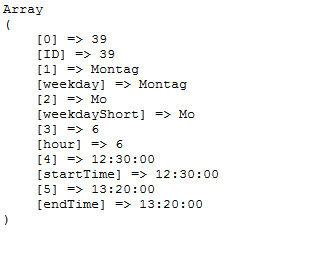
\includegraphics[keepaspectratio=true, width=8cm]{images/screenshots/content_mysql_fetch_row.png}
\caption{MySQL Zeile}
\label{fig:content_mysql_fetch_row}
\end{figure}
\begin{figure}[H]
\centering
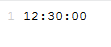
\includegraphics[keepaspectratio=true, width=3cm]{images/screenshots/content_mysql_fetch_column.png}
\caption{MySQL Spalte}
\label{fig:content_mysql_fetch_column}
\end{figure}